\scanpage{17}
\mspage{8}
$\mathcal Z_i\subset\mathcal X_i$ and $Z\simeq\mathcal Z_1$, $Z\simeq\mathcal Z_2$).

\uline{NB} One should note that contrary to what happens in $\deleted{\unsure{\operatorname{Cat}}}\inserted{\operatorname{Esp}}_{\mathcal M_*}$) a subobject of an object $\mathcal X$ of $\underrightarrow{\operatorname{Esp}}_{\mathcal M_*}$ i.e. of an ind-tame space, does not necessarily correspond to a $\mathrm{loc}^{\mathrm t}$ tame subset\ldots

\figure{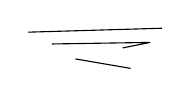
\begin{tikzpicture}\draw (0,0)--(1.7,.05);\draw (.3,-.15)--(1.55,-.13)--(1.2,-.2);\draw (.6,-.34)--(1.3,-.46);\end{tikzpicture}}
\figure{\begin{tikzpicture}\node[draw,ellipse] {$\overline{\underline{\mathrm V}}$};\end{tikzpicture}}
\uline{\unsure{Relations|Relation} to topologies} Suppose $R$ equipped with a topology, hence the $R^I$ and the tame ``models'' too. One would like the tame maps to be continuous --- this is OK if the tame subsets are compact (hence closed, if $R$ Hausdorff), this is the case. \deleted{If the functor $X\mathrel{\mapstochar\relbar}$} \inserted{Suppose therefore}
\figure{\begin{tikzpicture}\node[draw,ellipse] {$M9$};\end{tikzpicture}}
\[
 \left\{\begin{array}{l}R\text{ Hausdorff}\\
 \text{the tame subsets of }R^n\text{ are compact}
 \end{array}\right.
\]
Then the functor $X\mathbin{-}|X|$ factors through the category of topological spaces
\[
 \operatorname{Esp}_{\mathcal M_*}\longrightarrow(\deleted{\unsure{R|E}}\inserted{\mathrm E}\mathrm{sp.\ top.\ cpts})
\]
\mspage{16}
